\documentclass[11pt,letter]{article}

\usepackage{poma_style}

%%%%%% SYMBOLES %%%%%
\usepackage{tipa}	% pour avoir l'accent concave
\usepackage{nth} 	% pour avoir first, second ... : \nth{num}

%%%%%% EQUATION %%%%%%
\usepackage{amssymb}
\usepackage{amsmath}
\usepackage{fancybox}
\usepackage{xfrac}	% fraction de type "1/4"
\usepackage{cases}	% système équation
\usepackage[overload]{empheq}
\usepackage{bm}		% pour mettre en gras .
\usepackage{units} 	% x/y barre latérale pour les fractions

%%%%%% FIGURE %%%%%%
\usepackage{graphicx}	% insérer des graphiques
\usepackage{subfigure}	% utiliser subfigure
\usepackage{float}	% utiliser H dans les figures

%%%%%% TABLEAUX %%%%%%
\usepackage{array,multirow,makecell}
\usepackage{slashbox} % pour les \backslashbox
%\usepackage{subcaption}
\usepackage{hhline}	% pour les lignes horizontales 
\usepackage{xcolor,colortbl}

\newcolumntype{L}[1]{>{\raggedright\let\newline\\\arraybackslash\hspace{0pt}}m{#1}}
\newcolumntype{C}[1]{>{\centering\let\newline\\\arraybackslash\hspace{0pt}}m{#1}}
\newcolumntype{R}[1]{>{\raggedleft\let\newline\\\arraybackslash\hspace{0pt}}m{#1}}

%%%%%%%%%%%%%%%%%%%%%
\usepackage{url}	% gérer les adresses www.

\newcommand{\eps}{\varepsilon}


\begin{document}


%\section*{Abstract}
%
%Monitoring the acoustic urban environment is beneficial for improving the life of citizens. To do so, the research community in acoustics can benefit from corpora where the acoustic contribution of sources of disturbance such as road traffic is precisely known.
%
%In this paper, a set of urban sound mixtures are simulated using an open source tool \textit{simScene}. Their characteristics (type of sources, density of events, etc.) are inferred from the listening of reference audio scenes recorded in Paris, France. The main advantage of the simulated versions is that several quantities (such as the acoustic level of each source, a useful feature automated analysis tools) is precisely known.
%
%In order to quantify the level of realism achieved by the use of the simulation tool a perceptive test is conducted with 50 subjects. The results show that no significant differences can be made between the simulated and the recorded scenes.

\section{Introduction}

The urban sound environment is studied both from the perceptual \cite{jin_yong_soundwalk_2013} \cite{botteldooren_understanding_2011} and from the physical point of view \cite{can_describing_2015} \cite{raimbault_ambient_2003}. These studies can be based on real sound environments either by acoustic listening through a \textit{soundwalk} \cite{adams_soundwalking_2008} or with recordings made in city \cite{botteldooren_temporal_2006}, or in a laboratory by using sound mixtures resulting from a simulation process \cite{lafay_new_2014}. In the first case, since it has an undeniable ecological validity, it doesn't make it possible to have a repeatable experience nor to propose a controlled framework where the presence and the level of the different sound sources can be adjusted. Then the use of a simulation tool to create specific urban sound environments is a useful way to control the degree of contribution of each class of acoustical sources. It allows us to create urban sound environments by adjusting some parameters \cite{bruce_development_2009} or to evaluate performances of some classification or detection tools \cite{giannoulis_detection_2013}.

A critical question is then to obtain scenes that are realistic enough to be considered simulated scenes as similar to some reference recordings. To do so, various methods have been proposed. The first approach would be to simulate completely a neighborhood taking into account the architecture of the buildings, the sound dynamics of the different sources present (car, voice, bird, bell \dots) and their propagation to a receptor, as proposed by \cite{cstb_simulation_2015}. If the first renderings are interesting, this method remains complex to implement.
A more straightforward approach composes sound mixtures from isolated sounds mixed together. The idea is to consider the urban sound environment as the sum of acoustic events, i.e. events with a sufficient sound level to be discernible, superposed to a sound background, i.e a sound constant on the sound mixture whose properties vary slowly during the scene. The difficulty here is to have a representative database of isolated sounds with a sufficient quality to not compromise the resulting sound quality and to sequence the acoustic events wisely.

The method proposed in \cite{misra_musical_2007} enables to resolve the first issue by extracting the acoustical events directly in real recordings and by manipulating them to re-use them in new mixtures. Since the tool has a sufficient number of parameters to control the sound event, their method is limited by the extraction phase: the overlapping between the acoustic events deteriorates the sounds and then the final rendering. Furthermore, the manipulations (duration, frequency range) can create artifacts that can deacrease the realism. In a similar way, the tool proposed by Davis and Bruce \cite{bruce_development_2009} enables to compose sound mixtures with an isolated sound database composed of recordings made specially for their application. The creation of the urban sound mixtures is made possible with the perceptual evaluation of a panel of listeners of the different sound environments. This method enables to determine which sounds are the most representative or the most linked to an urban sound environment from a perceptual point of view.

However, as our objective here is to get simulated scenes that are as realistic as possible, this method can not be considered because if this method proposes a perceptual validity, it can not provide an ecological one. Thus, this study proposes to create urban sound mixtures from the listening of urban audio recordings and the estimation of some high level sequencing parameters extracted from the recordings to tune an audio simulation tool. The realism of the simulated scenes is then evaluated using a perceptual test.

The remaining of the paper is organized as follows: Section \ref{sec:study} focuses on the study of recordings made in Paris, Section \ref{sec:simulation} deals with the simulation tool and Section \ref{sec:test} summarizes the results obtained in the perspective test.


\section{Study of real scenes} \label{sec:study}
Real urban noise recordings are listened in details to determine the composition of typical urban sound environments in terms of sound sources, presence and level. The recordings considered in this study have been made on the \nth{13} district of Paris (France) as part of the GRAFIC project \cite{aumond_sound_2016} during a soundwalk which was designed to cover different types of urban sound environments.\\ 

\begin{figure}[H]
\centering
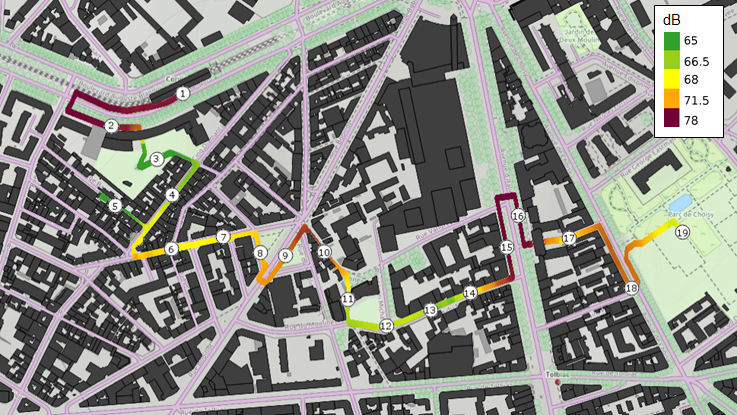
\includegraphics[width=.5\textwidth]{./pictures/trajet_19pts.png}
\caption{Map of the soundwalk with the 19 stop points}
\label{fig:soundwalk}
\end{figure}

The walk was 2.1 km long, consisting of 19 stop points with a recording duration between 3 to 5 minutes (see figure \ref{fig:soundwalk}). It was roamed on two days (03/23/2015 and 03/30/2015), twice a day (on the morning and on the afternoon) and in one direction (from West to East, WE) and then in the other (from East to West, EW). The acquisition system used was a ASAsense and was carried on the backpack of the operator which was walking with the participants. In the end, 76 (4 $\times$ 19) audio files (sampled at 44,1 kHz) were available and serve as a basis for the study. More details can be found on \cite{aumond_modelling_2017}. Each file is fully annotated in terms of sound classes that are present in the urban area and their recurrence. It is labeled using the following types of sound environments (\textit{park}, \textit{quiet street}, \textit{noisy street}, \textit{very noisy street}) as proposed by \cite{rychtarikova_soundscape_2013} or \cite{can_describing_2015} (Table~\ref{tab:classificationScene}).

\begin{table*}[h]
\centering

\begin{tabular}{|c|c|*{19}{l|}}
\hline
\multicolumn{1}{|l|}{\textbf{day}} & \textbf{journey}   & 1                        & 2                        & 3                        & 4                        & 5                        & 6                        & 7                        & 8                        & 9                        & 10                       & 11                       & 12                       & 13                       & 14                       & 15                       & 16                       & 17                       & 18                       & 19                       \\ \hline
\textbf{1} & \textbf{EW} & \cellcolor[HTML]{F56B00} & \cellcolor[HTML]{F56B00} & \cellcolor[HTML]{5AB25A} & \cellcolor[HTML]{FFCB2F} & \cellcolor[HTML]{FFCB2F} & \cellcolor[HTML]{F56B00} & \cellcolor[HTML]{FFCB2F} & \cellcolor[HTML]{5AB25A} & \cellcolor[HTML]{F56B00} & \cellcolor[HTML]{5AB25A} & \cellcolor[HTML]{FFCB2F} & \cellcolor[HTML]{F56B00} & \cellcolor[HTML]{FFCB2F} & \cellcolor[HTML]{FFCB2F} & \cellcolor[HTML]{F56B00} & \cellcolor[HTML]{9A0000} & \cellcolor[HTML]{FFCB2F} & \cellcolor[HTML]{F56B00} & \cellcolor[HTML]{5AB25A} \\
\hline
\textbf{1} & \textbf{WE} & \cellcolor[HTML]{F56B00} & \cellcolor[HTML]{F56B00} &                          & \cellcolor[HTML]{FFCB2F} & \cellcolor[HTML]{FFCB2F} & \cellcolor[HTML]{FFCB2F} & \cellcolor[HTML]{FFCB2F} & \cellcolor[HTML]{FFCB2F} & \cellcolor[HTML]{F56B00} & \cellcolor[HTML]{F56B00} & \cellcolor[HTML]{FFCB2F} & \cellcolor[HTML]{F56B00} & \cellcolor[HTML]{FFCB2F} & \cellcolor[HTML]{FFCB2F} & \cellcolor[HTML]{9A0000} & \cellcolor[HTML]{9A0000} & \cellcolor[HTML]{FFCB2F} & \cellcolor[HTML]{F56B00} &  \\
 \hline
\textbf{2} & \textbf{EW} & \cellcolor[HTML]{F56B00} & \cellcolor[HTML]{F56B00} & \cellcolor[HTML]{5AB25A} & \cellcolor[HTML]{FFCB2F} & \cellcolor[HTML]{FFCB2F} & \cellcolor[HTML]{FFCB2F} & \cellcolor[HTML]{FFCB2F} & \cellcolor[HTML]{FFCB2F} & \cellcolor[HTML]{F56B00} & \cellcolor[HTML]{F56B00} & \cellcolor[HTML]{FFCB2F} & \cellcolor[HTML]{F56B00} & \cellcolor[HTML]{FFCB2F} & \cellcolor[HTML]{F56B00} & \cellcolor[HTML]{9A0000} & \cellcolor[HTML]{9A0000} & \cellcolor[HTML]{FFCB2F} & \cellcolor[HTML]{F56B00} & \cellcolor[HTML]{5AB25A} \\
\hline
\textbf{2} & \textbf{WE} & \cellcolor[HTML]{F56B00} & \cellcolor[HTML]{F56B00} & \cellcolor[HTML]{5AB25A} & \cellcolor[HTML]{FFCB2F} & \cellcolor[HTML]{FFCB2F} & \cellcolor[HTML]{FFCB2F} & \cellcolor[HTML]{FFCB2F} & \cellcolor[HTML]{FFCB2F} & \cellcolor[HTML]{F56B00} & \cellcolor[HTML]{FFCB2F} & \cellcolor[HTML]{FFCB2F} & \cellcolor[HTML]{FFCB2F} & \cellcolor[HTML]{FFCB2F} & \cellcolor[HTML]{FFCB2F} & \cellcolor[HTML]{9A0000} & \cellcolor[HTML]{9A0000} & \cellcolor[HTML]{FFCB2F} & \cellcolor[HTML]{9A0000} & \cellcolor[HTML]{5AB25A} \\ \hline
\end{tabular}
%
\vspace{0.5cm}

\begin{tabular}{|p{1cm}|l|p{0.001cm}|p{2cm}|l|p{0.001cm}|p{2cm}|l|p{0.001cm}|p{2.75cm}|l|p{0.001cm}|p{2cm}|l|}

\hhline{|-|-|~|-|-|~|-|-|~|-|-|~|-|-|}
park & {\cellcolor[HTML]{5AB25A}} & & quiet street & {\cellcolor[HTML]{FFCB2F}} & & noisy street & {\cellcolor[HTML]{F56B00}} & &  very noisy street & {\cellcolor[HTML]{9A0000}} & & unclassified & \\
\hhline{|-|-|~|-|-|~|-|-|~|-|-|~|-|-|}

\end{tabular}

\caption{Classification of the scenes according to the sound environment}
\label{tab:classificationScene}
\end{table*}

Most of the scenes of the recordings belong to \textit{quiet street} and \textit{noisy street}. 2 scenes are removed form the database: a noisy cleaning truck is present inside the \textit{1-WE-3} heavily polluting the sound scene and the \textit{1-WE-19} record is too short to be considered in this study. From the annotations, each sound environment is characterized by the sound classes present in the recordings. The most recurrent sound classes are presented in Table \ref{tab:obsScene}.\\


\begin{table*}[!h]
\centering
\begin{tabular}{L{2.5cm} | C{2.5cm} | c | C{3cm} | C{2.5cm}}
\centering \textbf{Sound environment} & \textbf{Sound level (dB)} & \textbf{Background                                                       } &\textbf{Event} & \textbf{number events/min} \\ \hline
Park              & 69.0        &
\begin{tabular}[c]{@{}l@{}}voice, \\ bird's whistles\end{tabular} &
\begin{tabular}[c]{@{}l@{}}road traffic \\ voices\\ bird's whistle\\ street noise\\ foot step\end{tabular}                                         &
\begin{tabular}[c]{@{}l@{}}0.5\\ 0.5\\ 0.5\\ 0.5\\ 0.3\end{tabular}                       \\\hline
Quiet street      & 70.2        &
\begin{tabular}[c]{@{}l@{}}road traffic\\ bird\end{tabular}       &
\begin{tabular}[c]{@{}l@{}}road traffic \\ voices\\ street noises\\ foot step\\ bird\\ \begin{tabular}[c]{@{}l@{}}construction \\ \hfill site noise \end{tabular}\\ door house\\ door car\end{tabular} &
\begin{tabular}[c]{@{}l@{}}1.0\\ 0.7\\ 0.7\\ 0.5\\ 0.2\\ \begin{tabular}[c]{@{}l@{}} 0.1\\~\end{tabular}\\  0.2\\ 0.2\end{tabular}
\\ \hline
Noisy street      & 73.5        & road traffic                                                      & \begin{tabular}[c]{@{}l@{}}traffic\\ foot step\\ voice\\ street noise\\ bell\\ bird\\ car horn\\ car's door\\ siren\end{tabular}                   & \begin{tabular}[c]{@{}l@{}}9.0 \\ 0.5\\ 0.6\\ 0.4\\ 0.1\\ 0.2\\ 0.3\\ 0.2\\ 0.1\end{tabular} \\ \hline
Very noisy street & 76.0        & road traffic                                                      & \begin{tabular}[c]{@{}l@{}}traffic\\ voice\\ siren\\ car horn\\ bird\\ foot step\\ car's door\\ street noise\end{tabular}                          & \begin{tabular}[c]{@{}l@{}}40\\ 0.3\\ 0.2\\ 0.3\\ 0.2\\ 0.3\\ 0.2\\ 0.3\end{tabular}
\end{tabular}
\caption{Sound level and description of the most recurrent sound classes (backgrounds and events) present in the sound environments}
\label{tab:obsScene}
\end{table*}

As the calibration audio file was not available, the sound level cannot be considered as absolute but the relative difference between each sound environment can be considered. The road traffic, the voice and the bird components are the most discriminant classes of the sound environment: with exclusively road traffic, the \textit{noisy} and \textit{very noisy} environments sound environments are different to the \textit{park} and \textit{quiet street} where the voice and the bird's whistles are predominant. Furthermore, multiple sound classes can be heard whatever the urban sound environments : dog barks, church bell ringing, car horn, sirens \dots with a density that can be very low (< 0.1/min). Finally, a lot of brief sounds with unknown origin can be listened in almost all the files. Consequently, all these indefinite sounds are annotated in one unique class sound, \textit{street noise}. From this information (density, level, sound classes present in each sound environment), it is now possible to compose urban sound mixtures.

\section{Simulation of realistic auditory urban scenes} \label{sec:simulation}
\subsection{Presentation of the web-simulator \textit{simScene}}
\textit{simScene} \cite{rossignol_simscene:_2015} is a simulator that creates sound mixtures in a .wav format by superposing audio samples that come from an isolated sound database composed of two categories: the brief sounds (from 1 to 20 seconds) that are considered as salient belong to the \textit{event} category whereas all the sound that are of long duration and whose acoustic properties do not vary with respect to time belong to the \textit{background} category. Inside each category, the sound samples are then grouped in sound classes (bird, car, foot steps \dots). The software enables the user to control for each sound class some parameters as the number of events of each class that appears in the mixture, the elapsed time between each sample of a same class or the existence of a fade in and a fade out \dots. Each parameter is completed with a standard deviation that may brings some random behavior between the scenes. \\


\begin{figure}[h]
\centering
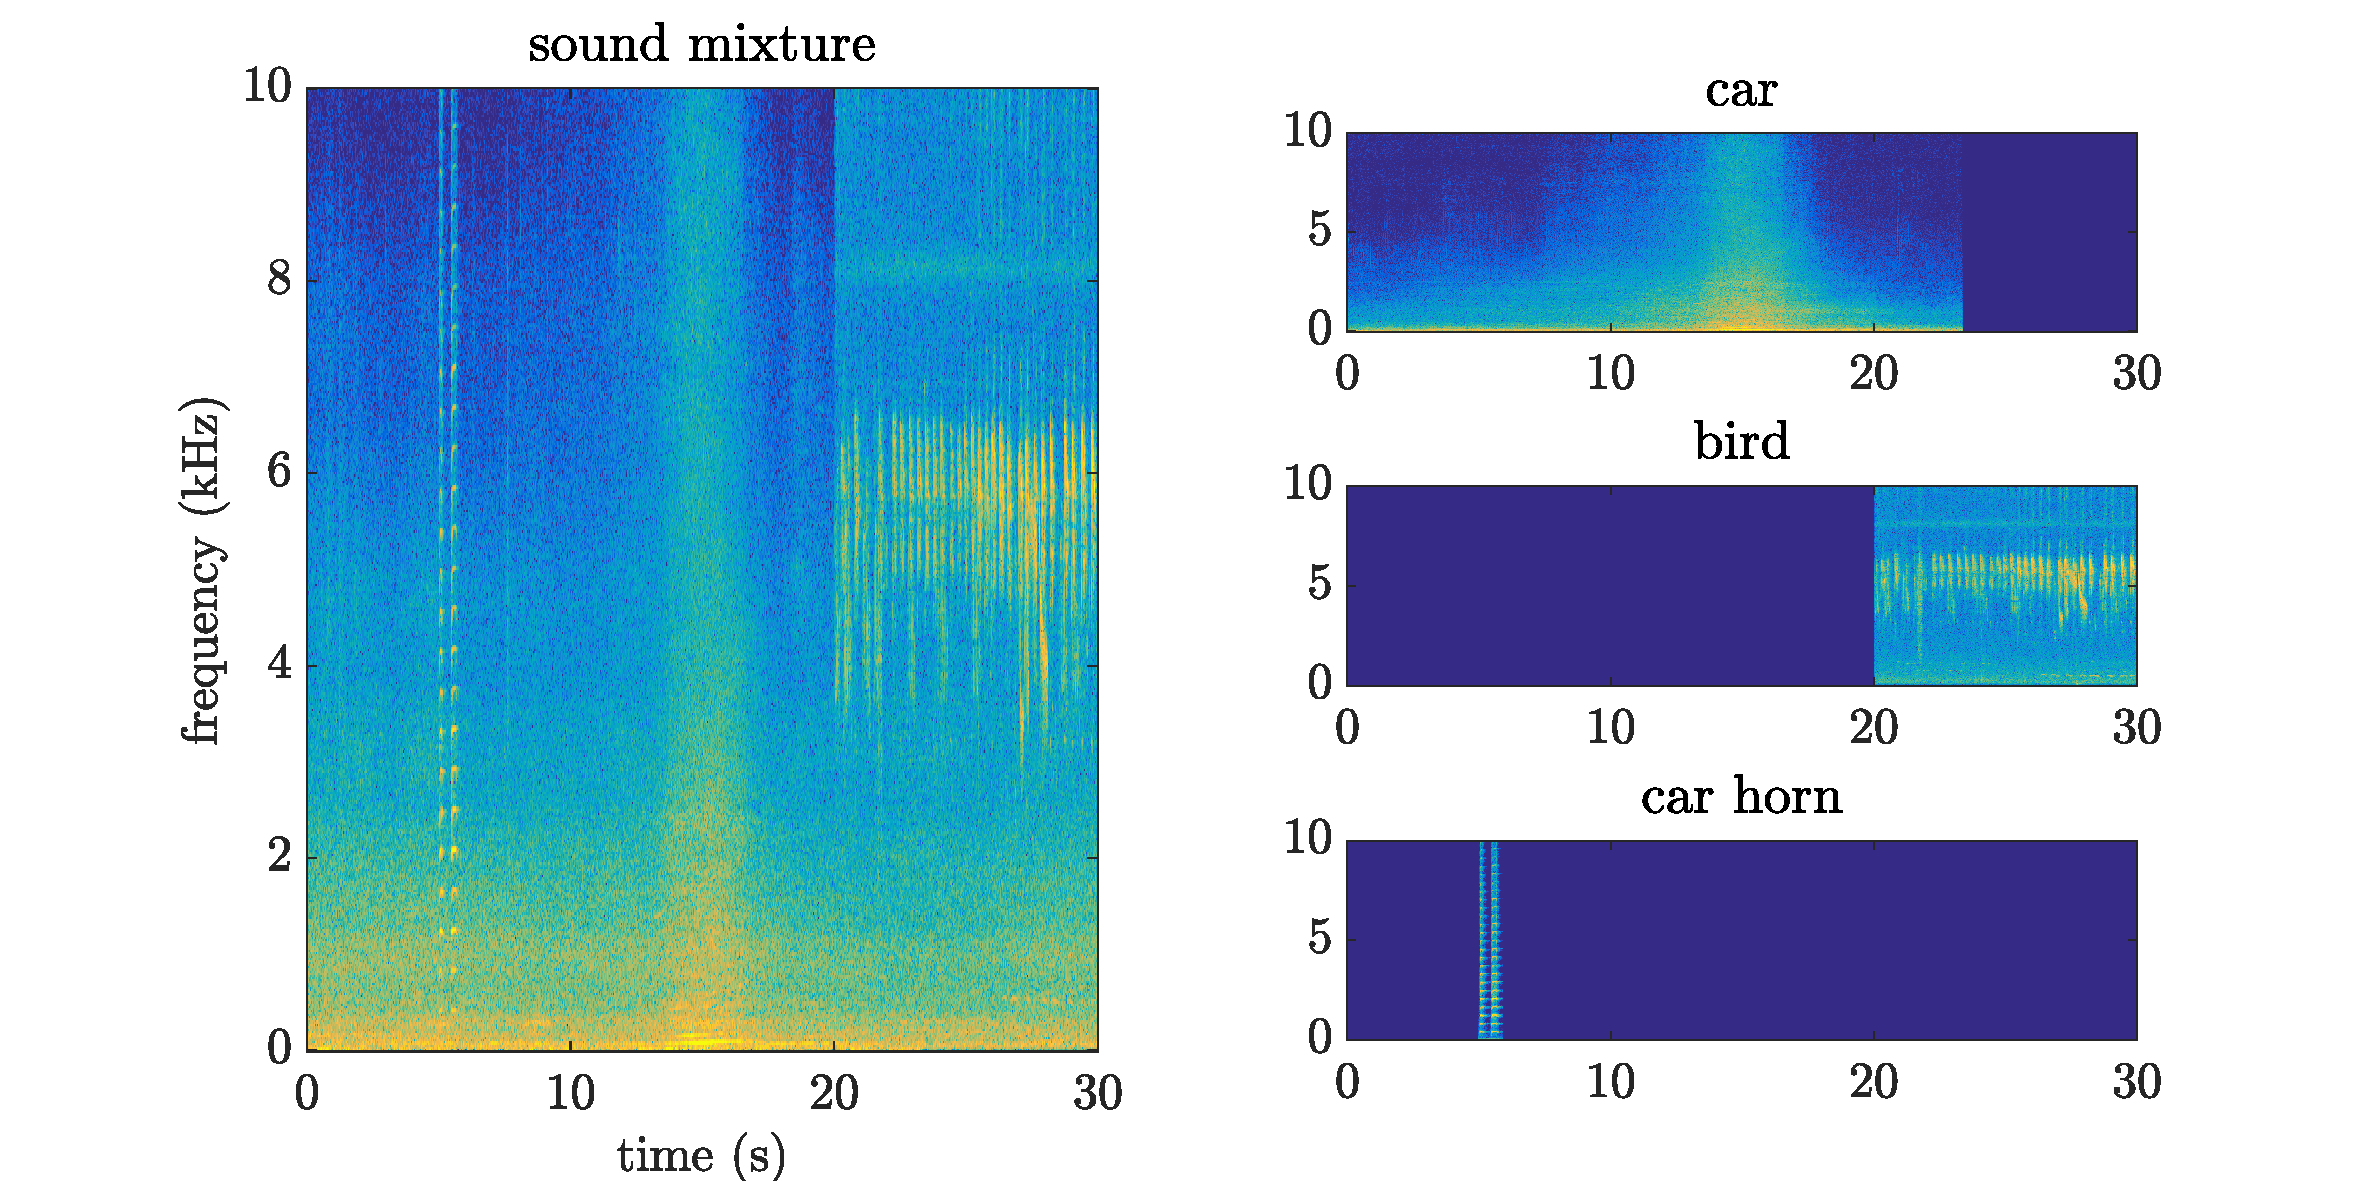
\includegraphics[width = .7\linewidth]{./pictures/spectrogramme_abstract_sceneSimpleKlaxonFixe_EN.pdf}
\caption{Example of a scene composed of three sound classes}
\label{fig:exampleSimScene}
\end{figure}


The sound mixtures can be created following two modes: the \textit{abstract} mode allows to create mixtures from the specified parameters while the \textit{replicate} mode reproduces an existing scene by following as much as possible its annotation file. With the audio file of the global sound mixture, each sound class can be resumed in a separate audio file, which allows to know their exact contribution in the scene. 

\subsection{Creation of the urban sound database}
Based on the annotations of the 74 real scenes, a sound database is built using the \textit{replicate} mode of \textit{simScene} with sounds found online on the \textit{freesound} project and with the help of the urbanSound8k database \cite{salamon_dataset_nodate}. This database consists in more than 8000 files with a 4 seconds or less duration, found on the web site freesound.org too, and classified in 10 sound classes : ventilation, car horn, children playing, dog barking, bell, engine idling, gunshot, jackhammer, siren and street music. All the audio files have been sorted and those who presented the best signal to noise ratio have been selected.\\

In addition, as road traffic is a prime audio source in an urban sound environment, it seemed interesting to have, in the database, a part composed of well-recorded car sounds. As a result, passages of 4 different cars (Renault Scenic, Clio, Megane and Dacia Sandero) were recorded on the Ifsttar-Nantes runway at different speeds and gear ratios for steady, acceleration, braking (Table~\ref{tab:resum_car_audio}) and stopped phases. Among the 108 recordings planned, those for the acceleration and braking phase for the Renault Senic could not be done whereas some recordings have been made twice for the other vehicles. In all, 103 car passages have been recorded. \\

\begin{table*}[!htb]
    \begin{minipage}{.5\linewidth}
      \centering
        \begin{tabular}{|c|c|lllll}
\cline{2-7}
\multicolumn{1}{l|}{} & \multicolumn{1}{l|}{\textbf{Trans.}} & \multicolumn{1}{l|}{\textbf{1}} & \multicolumn{1}{l|}{\textbf{2}} & \multicolumn{1}{l|}{\textbf{3}} & \multicolumn{1}{l|}{\textbf{4}} & \multicolumn{1}{l|}{\textbf{5}} \\ \hline
\multicolumn{1}{|c|}{\multirow{8}{*}{\begin{tabular}[c]{@{}c@{}}\textbf{stabilized}\\   \textbf{speed}\\   \textbf{(km/h)}\end{tabular}}} & \textbf{20} & \multicolumn{1}{l|}{$\times$} & \multicolumn{1}{l|}{} & \multicolumn{1}{l|}{} & \multicolumn{1}{l|}{} & \multicolumn{1}{l|}{} \\ \cline{2-7}
\multicolumn{1}{|c|}{} & \textbf{30} & \multicolumn{1}{l|}{} & \multicolumn{1}{l|}{$\times$} & \multicolumn{1}{l|}{$\times$} & \multicolumn{1}{l|}{} & \multicolumn{1}{l|}{} \\ \cline{2-7}
\multicolumn{1}{|c|}{} & \textbf{40} & \multicolumn{1}{l|}{} & \multicolumn{1}{l|}{$\times$} & \multicolumn{1}{l|}{$\times$} & \multicolumn{1}{l|}{$\times$} & \multicolumn{1}{l|}{} \\ \cline{2-7}
\multicolumn{1}{|c|}{} & \textbf{50} & \multicolumn{1}{l|}{} & \multicolumn{1}{l|}{} & \multicolumn{1}{l|}{$\times$} & \multicolumn{1}{l|}{$\times$} & \multicolumn{1}{l|}{} \\ \cline{2-7}
\multicolumn{1}{|c|}{} & \textbf{60} & \multicolumn{1}{l|}{} & \multicolumn{1}{l|}{} & \multicolumn{1}{l|}{} & \multicolumn{1}{l|}{$\times$} & \multicolumn{1}{l|}{$\times$} \\ \cline{2-7}
\multicolumn{1}{|c|}{} & \textbf{70} & \multicolumn{1}{l|}{} & \multicolumn{1}{l|}{} & \multicolumn{1}{l|}{} & \multicolumn{1}{l|}{$\times$} & \multicolumn{1}{l|}{$\times$} \\ \cline{2-7}
\multicolumn{1}{|c|}{} & \textbf{80} & \multicolumn{1}{l|}{} & \multicolumn{1}{l|}{} & \multicolumn{1}{l|}{} & \multicolumn{1}{l|}{} & \multicolumn{1}{l|}{$\times$} \\ \cline{2-7}
\multicolumn{1}{|c|}{} & \textbf{90} & \multicolumn{1}{l|}{} & \multicolumn{1}{l|}{} & \multicolumn{1}{l|}{} & \multicolumn{1}{l|}{} & \multicolumn{1}{l|}{$\times$} \\ \hline
\end{tabular}
    \end{minipage}
    \begin{minipage}{.5\linewidth}
      \centering
\begin{tabular}{|c|c||c|c|}
\hline
\multicolumn{2}{|c||}{\textbf{braking}} & \multicolumn{2}{|c|}{\textbf{acceleration}} \\ \hline
\multicolumn{1}{|c|}{\begin{tabular}[c]{@{}c@{}}\textbf{speed}\\  \textbf{(km/h)}\end{tabular}} & \multicolumn{1}{c||}{\textbf{gear r.}} & \multicolumn{1}{c|}{\begin{tabular}[c]{@{}c@{}}\textbf{speed}\\  \textbf{(km/h)}\end{tabular}} & \multicolumn{1}{c|}{\textbf{gear r.}} \\ \hline
50 $\rightarrow$ 0 & 3 $\rightarrow$ 2 & 0 $\rightarrow$ 30 & 1 $\rightarrow$ 2 \\ \hline
40 $\rightarrow$ 0 & 2 $\rightarrow$ 2 & 0 $\rightarrow$ 40 & 1 $\rightarrow$ 2 \\ \hline
50 $\rightarrow$ 30 & 3 $\rightarrow$ 2 & 20 $\rightarrow$ 40 & 1 $\rightarrow$ 3 \\ \hline
60 $\rightarrow$ 40 & 4 $\rightarrow$ 3 & 30 $\rightarrow$ 50 & 2 $\rightarrow$ 3 \\ \hline
70 $\rightarrow$ 50 & 4 $\rightarrow$ 3 & 40 $\rightarrow$ 60 & 3 $\rightarrow$ 4 \\ \hline
80 $\rightarrow$ 50 & \begin{tabular}[c]{@{}l@{}}4 or 5\\ $\rightarrow$ 3\end{tabular} & 50 $\rightarrow$ 70 & \begin{tabular}[c]{@{}l@{}}3 $\rightarrow$ \\ 4 or 5\end{tabular} \\ \hline
\end{tabular}
    \end{minipage}%
    \caption{Description of the recordings set on runway with vehicle passages with stabilized speed (left) and in acceleration and braking phase(right) with different gear ratios}
    \label{tab:resum_car_audio}
\end{table*}

To obtain the cleanest possible sound samples, a median filter \cite{fitzgerald_harmonic/percussive_2010} has to be applied to filter out bird's whistles present in the recordings. The filter consists in taking a window around a center point and to attribute to it the median value of this window. This method allows to attenuate the brief variations both in the spectral and the temporal plan. The size of the filter window is chosen with a 5 points width and a 9 points height in the frequency range $\left[ 2500-6500 \right]$ Hz, so that the effect of the filter is sufficient without deteriorating the quality of the audio (see Figure \ref{fig:filtre_car}).

\begin{figure}[hbtp]
\centering
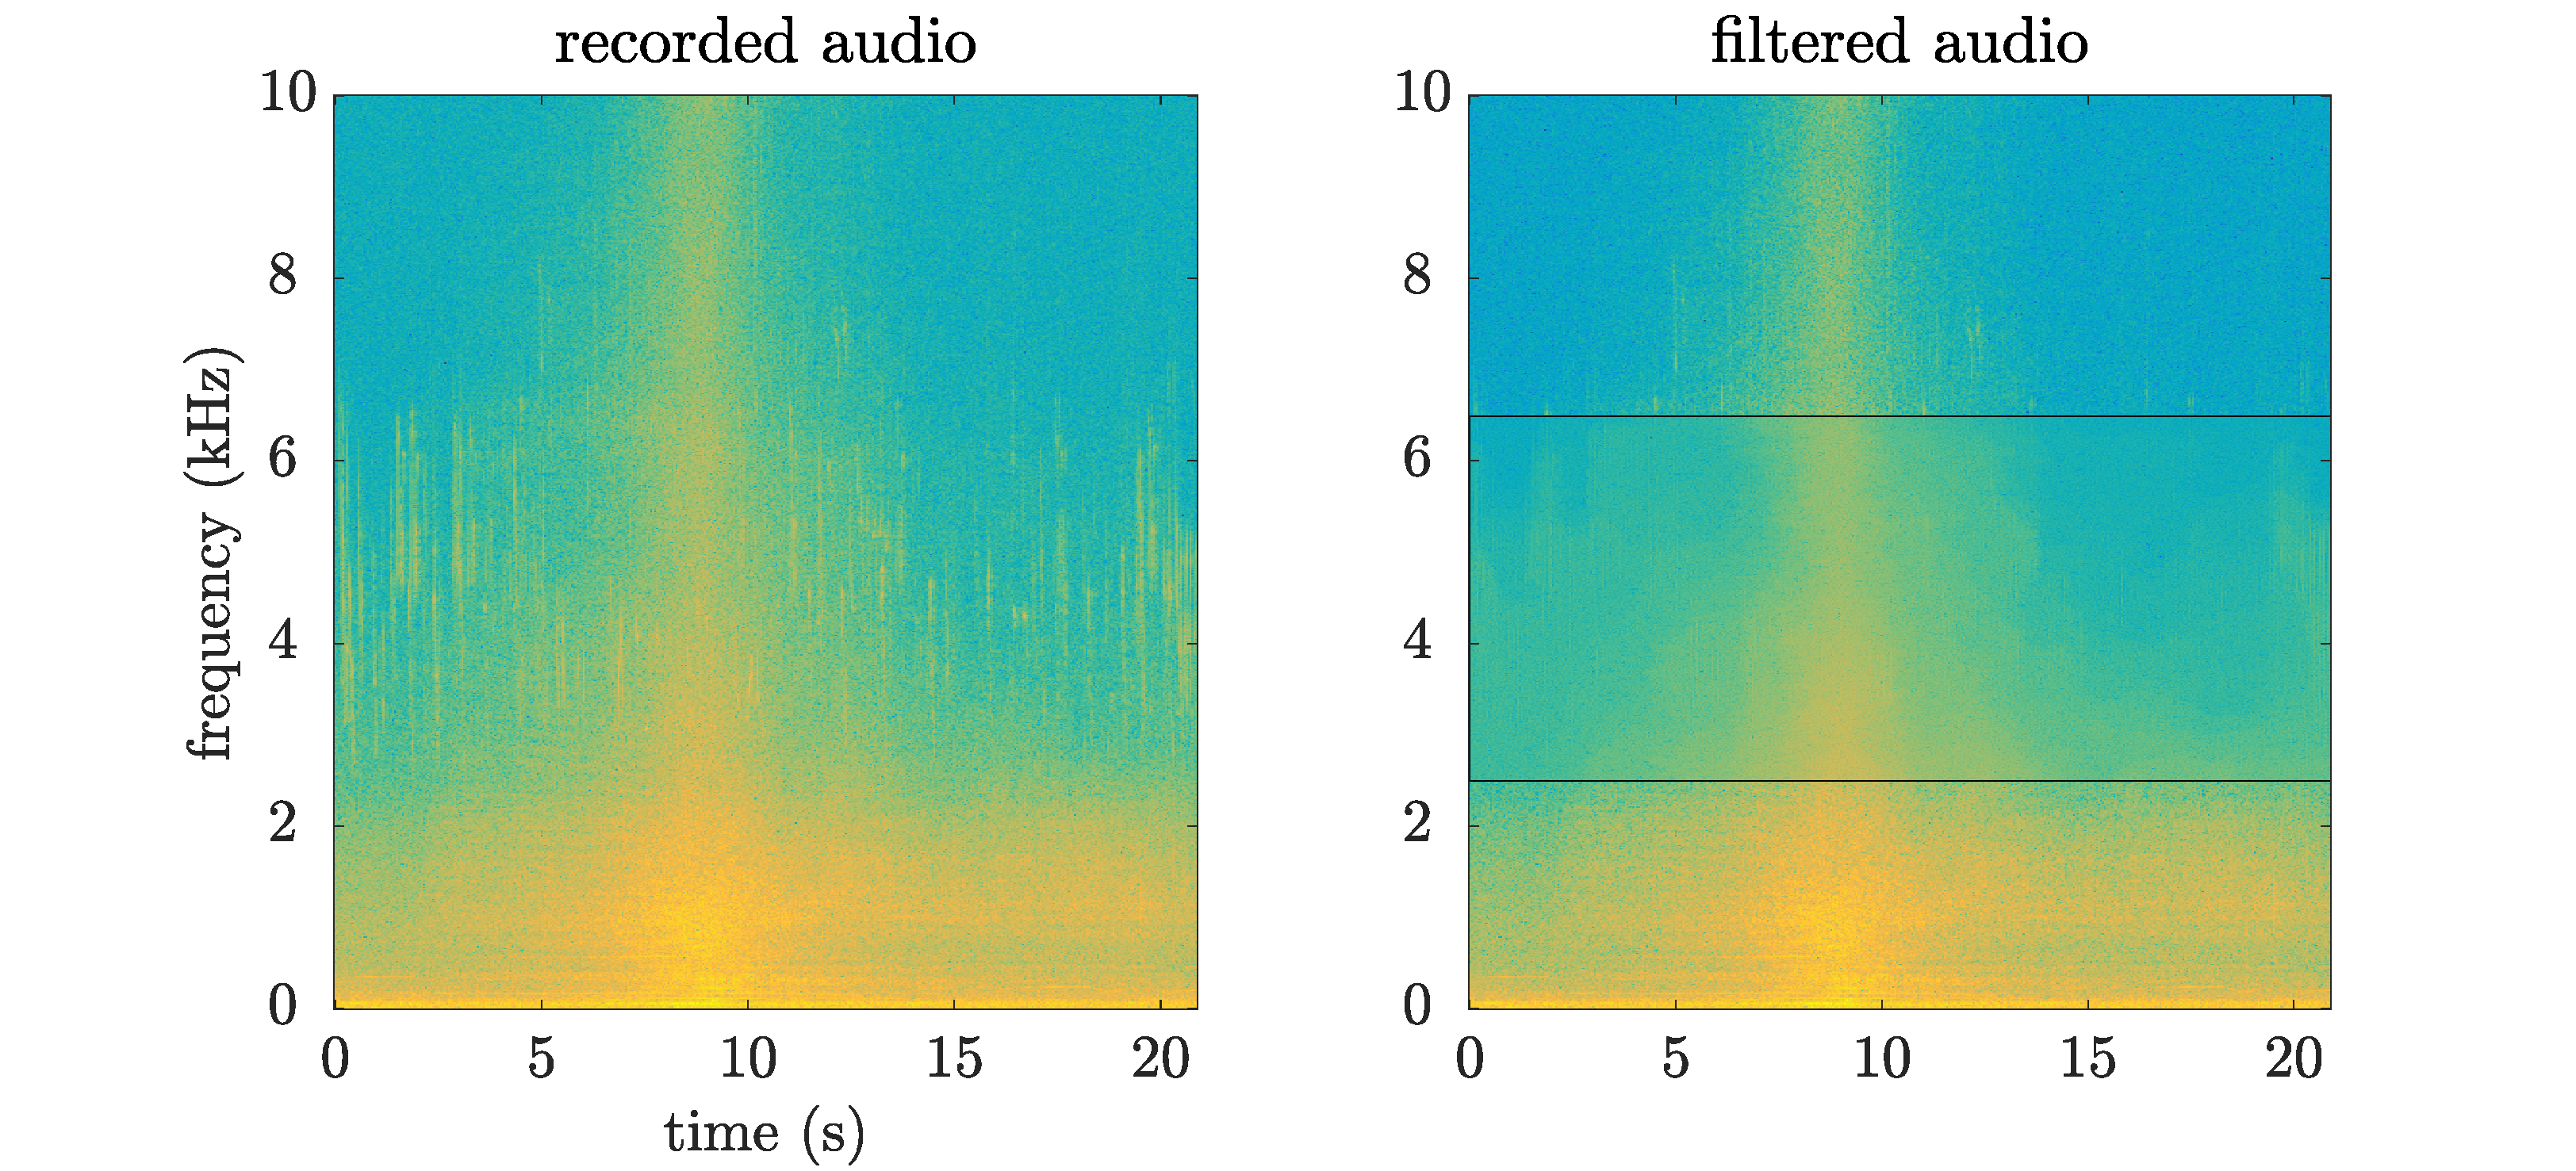
\includegraphics[width=.7\linewidth]{./pictures/filtrageMedian_VL1_R3_40_EN.pdf}
\caption{Spectrogram in the frequency range $\left[ 2500-6500 \right]$ Hz of a recorded passage of the Renault Megane car at 40 km/h with the \nth{3} gear ratio ($N_{w} = 2^{12}$ with 50 $\%$ overlapping, $N_{fft} = 2^{12}$, $sr = 44.1$ kHz). On the left, the original recording, on the right, the filtered audio with the filtered part.}
\label{fig:filtre_car}
\end{figure}

Finally, the resulting database is composed of 245 sound events (bell, whistle bird, sweeping broom, car horn, car, hammer and drill, coughing, dog barking, car and house door slamming, plane, siren, foot step, thunder, street noise, suitcase rolling, train and tramway passing, truck and voice) and of 154 background sounds (birds, construction site, crowd, park, rain, schoolyard, traffic, ventilation, wind). With this built-up database, the 74 real sound scenes are replicated. In order to obtain a corpus of urban sound scenes, resulting from a simulated process, sufficiently realistic, a perceptual test is set up to evaluate the realism on several of them.

\section{Perceptual test} \label{sec:test}
\subsection{Design of the test}
A perceptual test is conducted with a panel of listeners that are asked to evaluate the level of realism on a 7-point scale (1 is \textit{not realistic at all}, 7 is \textit{very realistic}) of an auditory scenes, recorded and simulated. The total number of sound scenes to be tested is set at 40. It consists of 20 30-seconds audio files, including 5 scenes that belong to the sound environment \textit{Park}, 6 from \textit{Quiet street}, 4 from \textit{Noisy street} and 5 from \textit{Very noisy street} chosen randomly among the 74 recorded scenes, and the same 30 seconds from the replicated scenes. In order to limit the duration of the test and to preserve the concentration of the subjects, each subject listens a subset of 20 sound scenes (10 real sounds scenes and 10 replicated). Furthermore, to prevent the listeners from changing the sound level of their speakers, all the scenes are normalized to the same sound level, chosen at 65 dB.\\

The experimental design is elaborated following a Balanced Incomplete Block Design (BIBD) \cite{dagnelie_principes_2003} where $J$ participants make $K$ evaluations from $B$ sound scenes, each of them are tested $R$ times and each couple of sound sources are presented $\lambda$ times in one block. In order to have BIBD, a 3 rules govern these parameters :

\begin{subequations}\label{eq:BIE_cond}
\begin{align}
B &\geq K, \label{eq:BIE_cond1}\\
JK &= BR, \label{eq:BIE_cond2}\\
\lambda &= R\frac{K-1}{B-1}. \label{eq:BIE_cond3}
\end{align}
\end{subequations}

with $\left[J, B, K, R, \lambda\right] \in \mathbb{N}$. A reasonable number of listeners is chosen at $J = 50$.  With theses parameters fixed, $J=50$, $K=20$, $B=40$ and $R=25$, the BIBD is not fully balanced (condition (\ref{eq:BIE_cond3}) $\notin \mathbb{N}$). It is finally with a partially BIBD that the listening plan is elaborated \cite{pages_blocs_2007}. It consists, with the parameters $J$, $K$ and $R$ fixed, in determining the optimal plan that would be the most balanced. The package \textit{sensoMineR} on the \textit{R} software provides the plan where the listening order per participant is defined inside \cite{le_sensominer:_2008}. As the distribution of the simulated and real samples for each participant is almost identical, the obtained listening plan can be considered as balanced (Figure \ref{fig:repartition}).\\

\begin{figure}[ht]
\centering
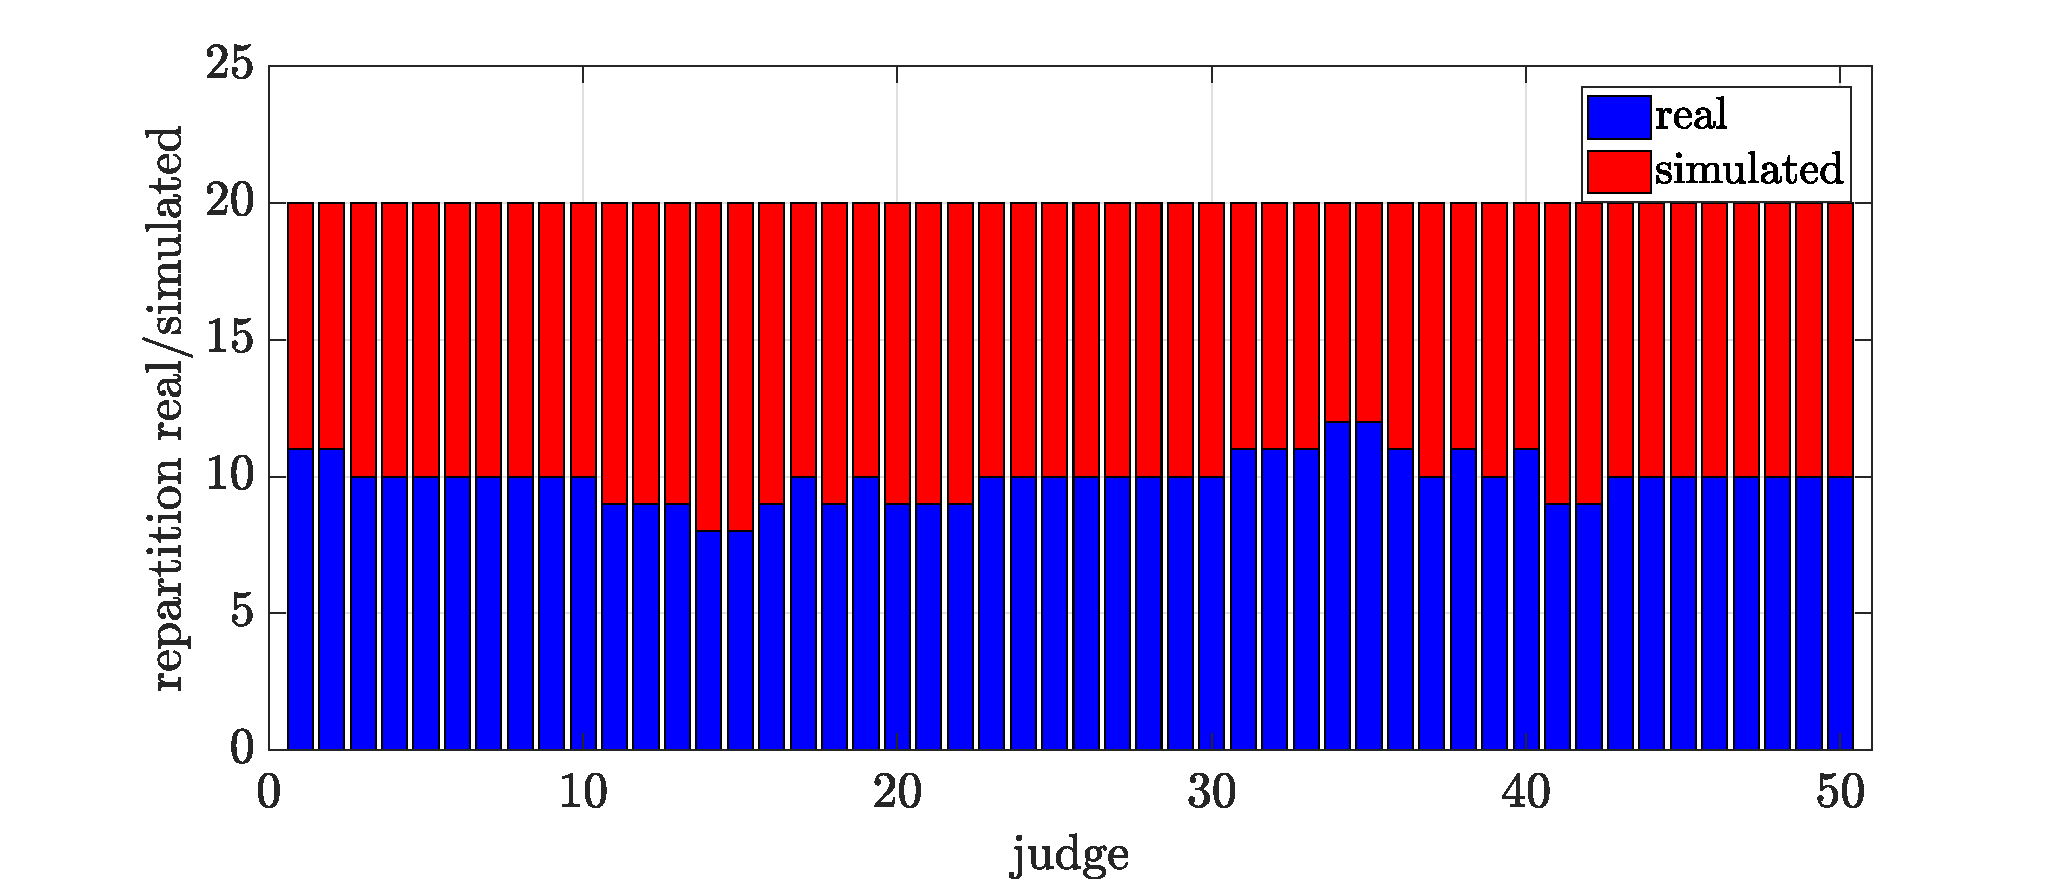
\includegraphics[width = .7\linewidth]{./pictures/repartition-real-simulated.pdf}
\caption{Distribution between the real and simulated scenes for each judge. The cumulative sum is equal to the number of tested elements $K$.}
\label{fig:repartition}
\end{figure}

The test was administered online\footnote{\url{http://soundthings.org/research/xpRealism}} on the 8 February 2017 and the number of 50 participants has been reached 12 days later. During the test, the participant had the possibility to listen to each scene as many times as wanted before evaluating it, without being able to change his/her judgment afterwards. The participant could also leave a comment on each audio to explain the rating. Finally, the age, gender and experience on listening to urban sound mixtures were asked at the end of the test. The panel of 50 listeners was made of 31 males and 18 females (one not documented) with an average age of 36 ($\pm$ 12) years old. $62\%$ of the participants declared having no experience in the listening of urban sound mixtures.\\

%\begin{figure}[ht]
%\centering
%\includegraphics[width=\linewidth]{../../../Pictures/test_perceptif/testPerceptif_panel.pdf}
%\caption{Description of the panel information}
%\label{fig:panel}
%\end{figure}



\subsection{Results}

First, the note distributions are represented by a box-and-whiskers plot according to whether they belongs to the type 'real' or 'simulated'. 
\begin{figure}[hbtp]
\centering
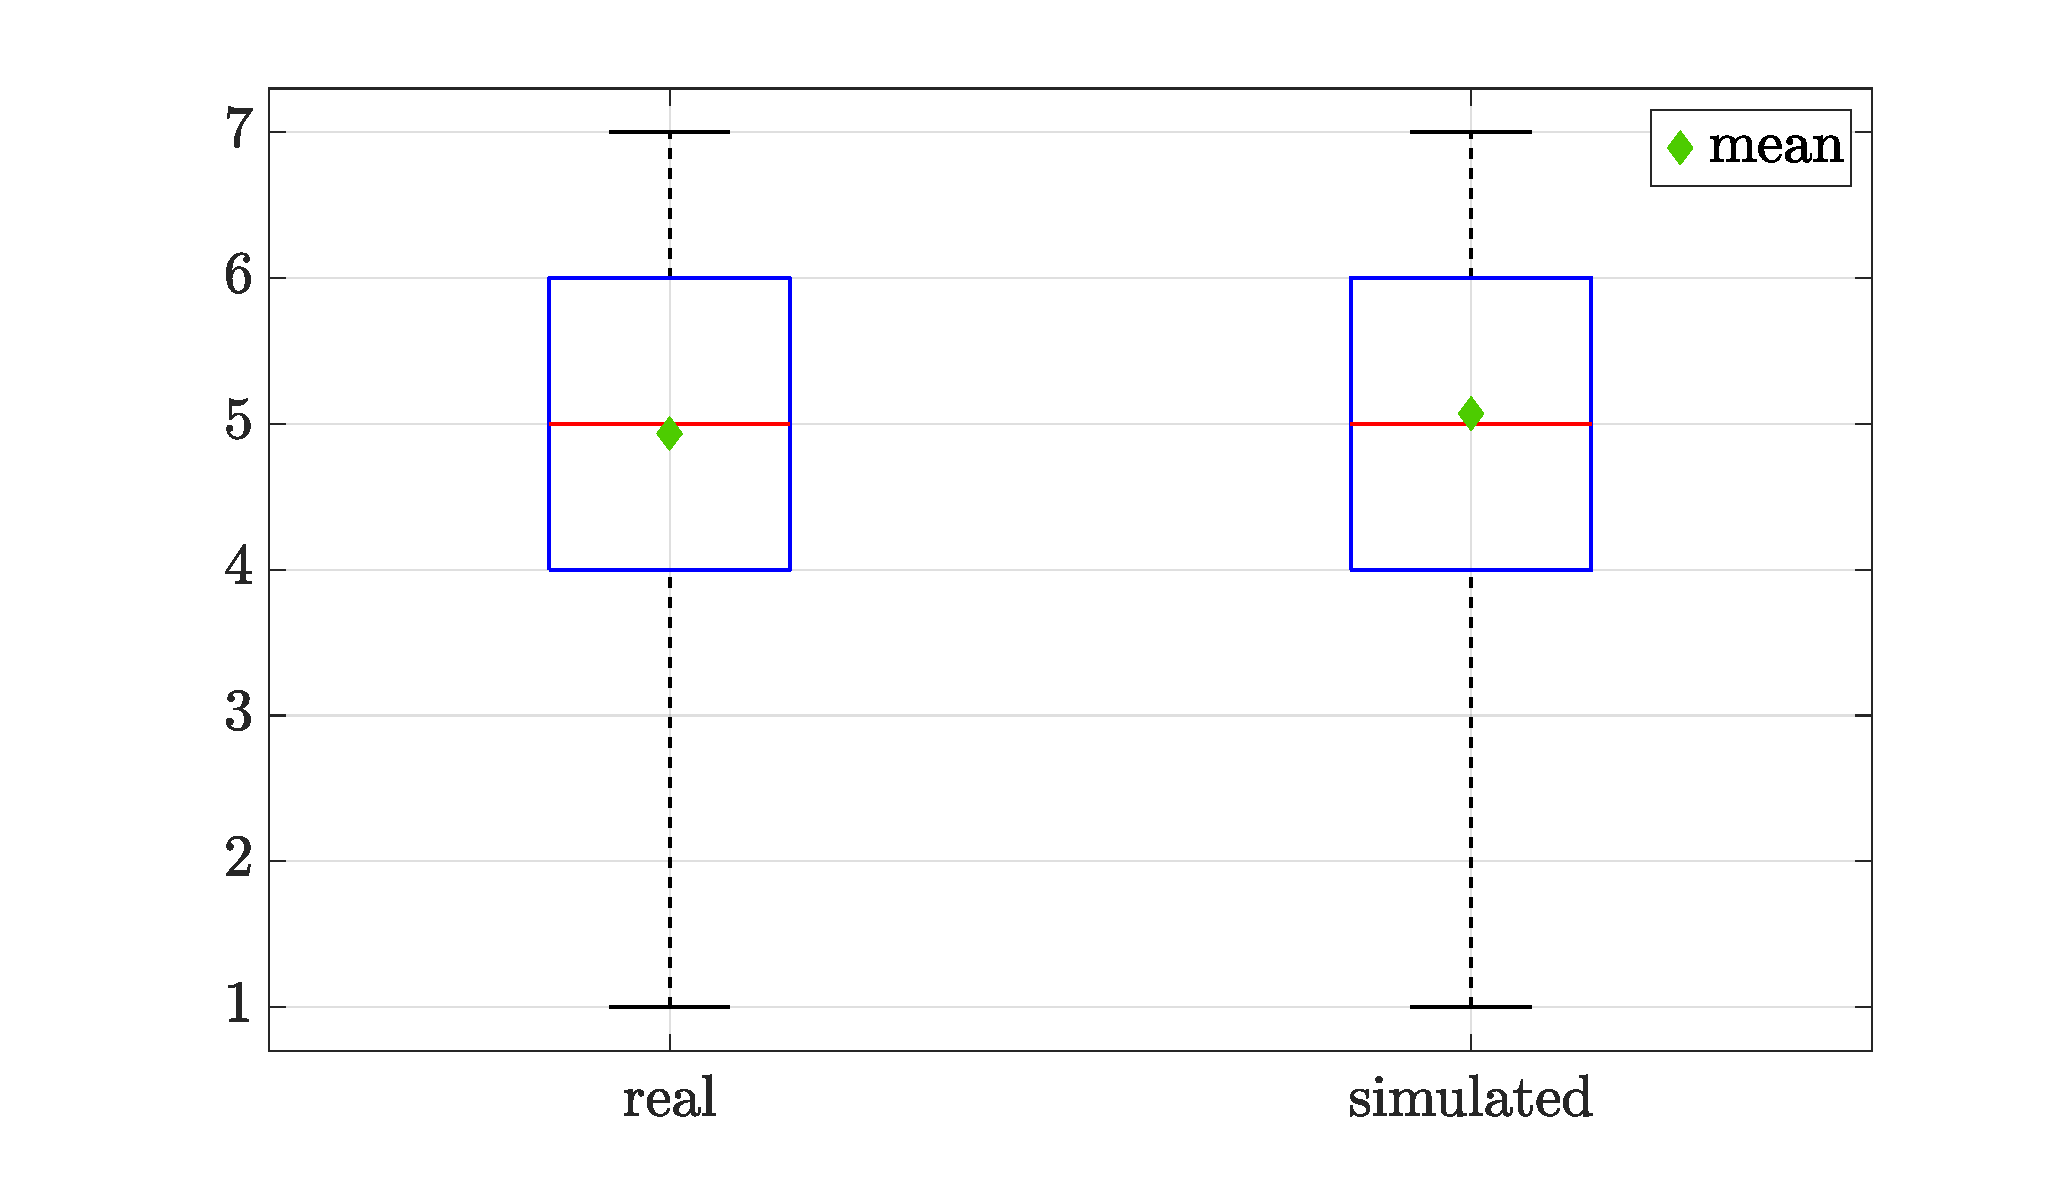
\includegraphics[width=.6\linewidth]{./pictures/testPerceptif_boxplotType_EN.pdf}
\caption{Box-and-whiskers plot of the rating of realism according to the type of scene}
\label{fig:boxplot_real_simul}
\end{figure}

The distribution allow to considered that the notation given the subjects are extremely similar. One can note that the mean for the simulated scene is even superior to the real one ($m_{simul.} = 5.1 (\pm 1.6$), $ m_{real} = 4.9 (\pm 1.6$)). 


A paired samples \textit{t-test} is then performed to validate the similarity between the two types. It consists in validate (or not) an $H_0$ hypothesis which considers the similarity between the distribution of the average scores for the recorded and the simulated scenes of each judge with a Student test. This test establishes a \textit{p-value} that is compared to a threshold value $\alpha$ of $5\%$. The $H_0$ hypothesis is then considered if $p-value > \alpha$. The results of the \textit{t-test} (degrees of freedom (DOF), the absolute value \textit{t} and \textit{p-value}) are sum up in the table \ref{tab:ttest_type_of_scene}.

\begin{table}[H]
\centering
\begin{tabular}{cccc}
        & DOF & \textit{$\mid$ t $\mid$}    & \textit{p-value} \\ 
\hline
type & 49 & 1.37 &  0.17   \\
\hline
\end{tabular}
\caption{T-test performed on the distribution of the average scores for the recorded and simulated scenes}
\label{tab:ttest_type_of_scene}
\end{table}


The $p-value$ is calculated at $0.17 > \alpha$, which confirms that all the real and simulated scenes are perceived in a similar way by the panel.\\

From this global result, a first analyze of variance (ANOVA) is performed to determine if the experience in the listening of urban sound mixtures is an influential factor to distinguish real and replicated scenes. In a similar way than the \textit{t-test}, but based on a Fischer statistical test, an ANOVA allows to determine if the distribution of different level of multiple factors are similar. It allows too to take into account multiple factors and their interactions. Therefore, a two-way ANOVA with interaction with the factors 'experience of the panelist in the listening of urban sound scene' (yes or no) and 'type of scene' (real or simulated) is carried out.  The DOF, the Fisher statistics and the associated \textit{p-value} are given in Table~\ref{tab:ANOVA_type_exp}.\\

\begin{table}[h]
\centering
\begin{tabular}{cccc}
        & DOF & \textit{F-statistic}    & \textit{p-value} \\ 
\hline
type & 1 & 0.59 & 0.44 \\
\hline
experience  & 1 & 1.97 & 0.16 \\ 
\hline
type/exp. & 1 & 2.14 & 0.14 \\
\hline
\end{tabular}
\caption{Two-ways ANOVA with the factors 'type of sound' and 'listener experience'.}
\label{tab:ANOVA_type_exp}
\end{table}

The effect of each factors and the interaction between them are not significant (\textit{p-value} $>$ 0.05). This means that even listeners trained to hear urban sound environments do not dissociate the real scenes from the simulated scenes better than the non-experienced listeners.\\

The effect of the 'scene type' and the 'sound environment' factors and the interaction are then studied in a two-ways ANOVA (data distributions displayed on Figure \ref{fig:boxplot_type_ambience} and results in Table \ref{tab:p_value_type_ambience}).\\

\begin{figure}[h]
\centering
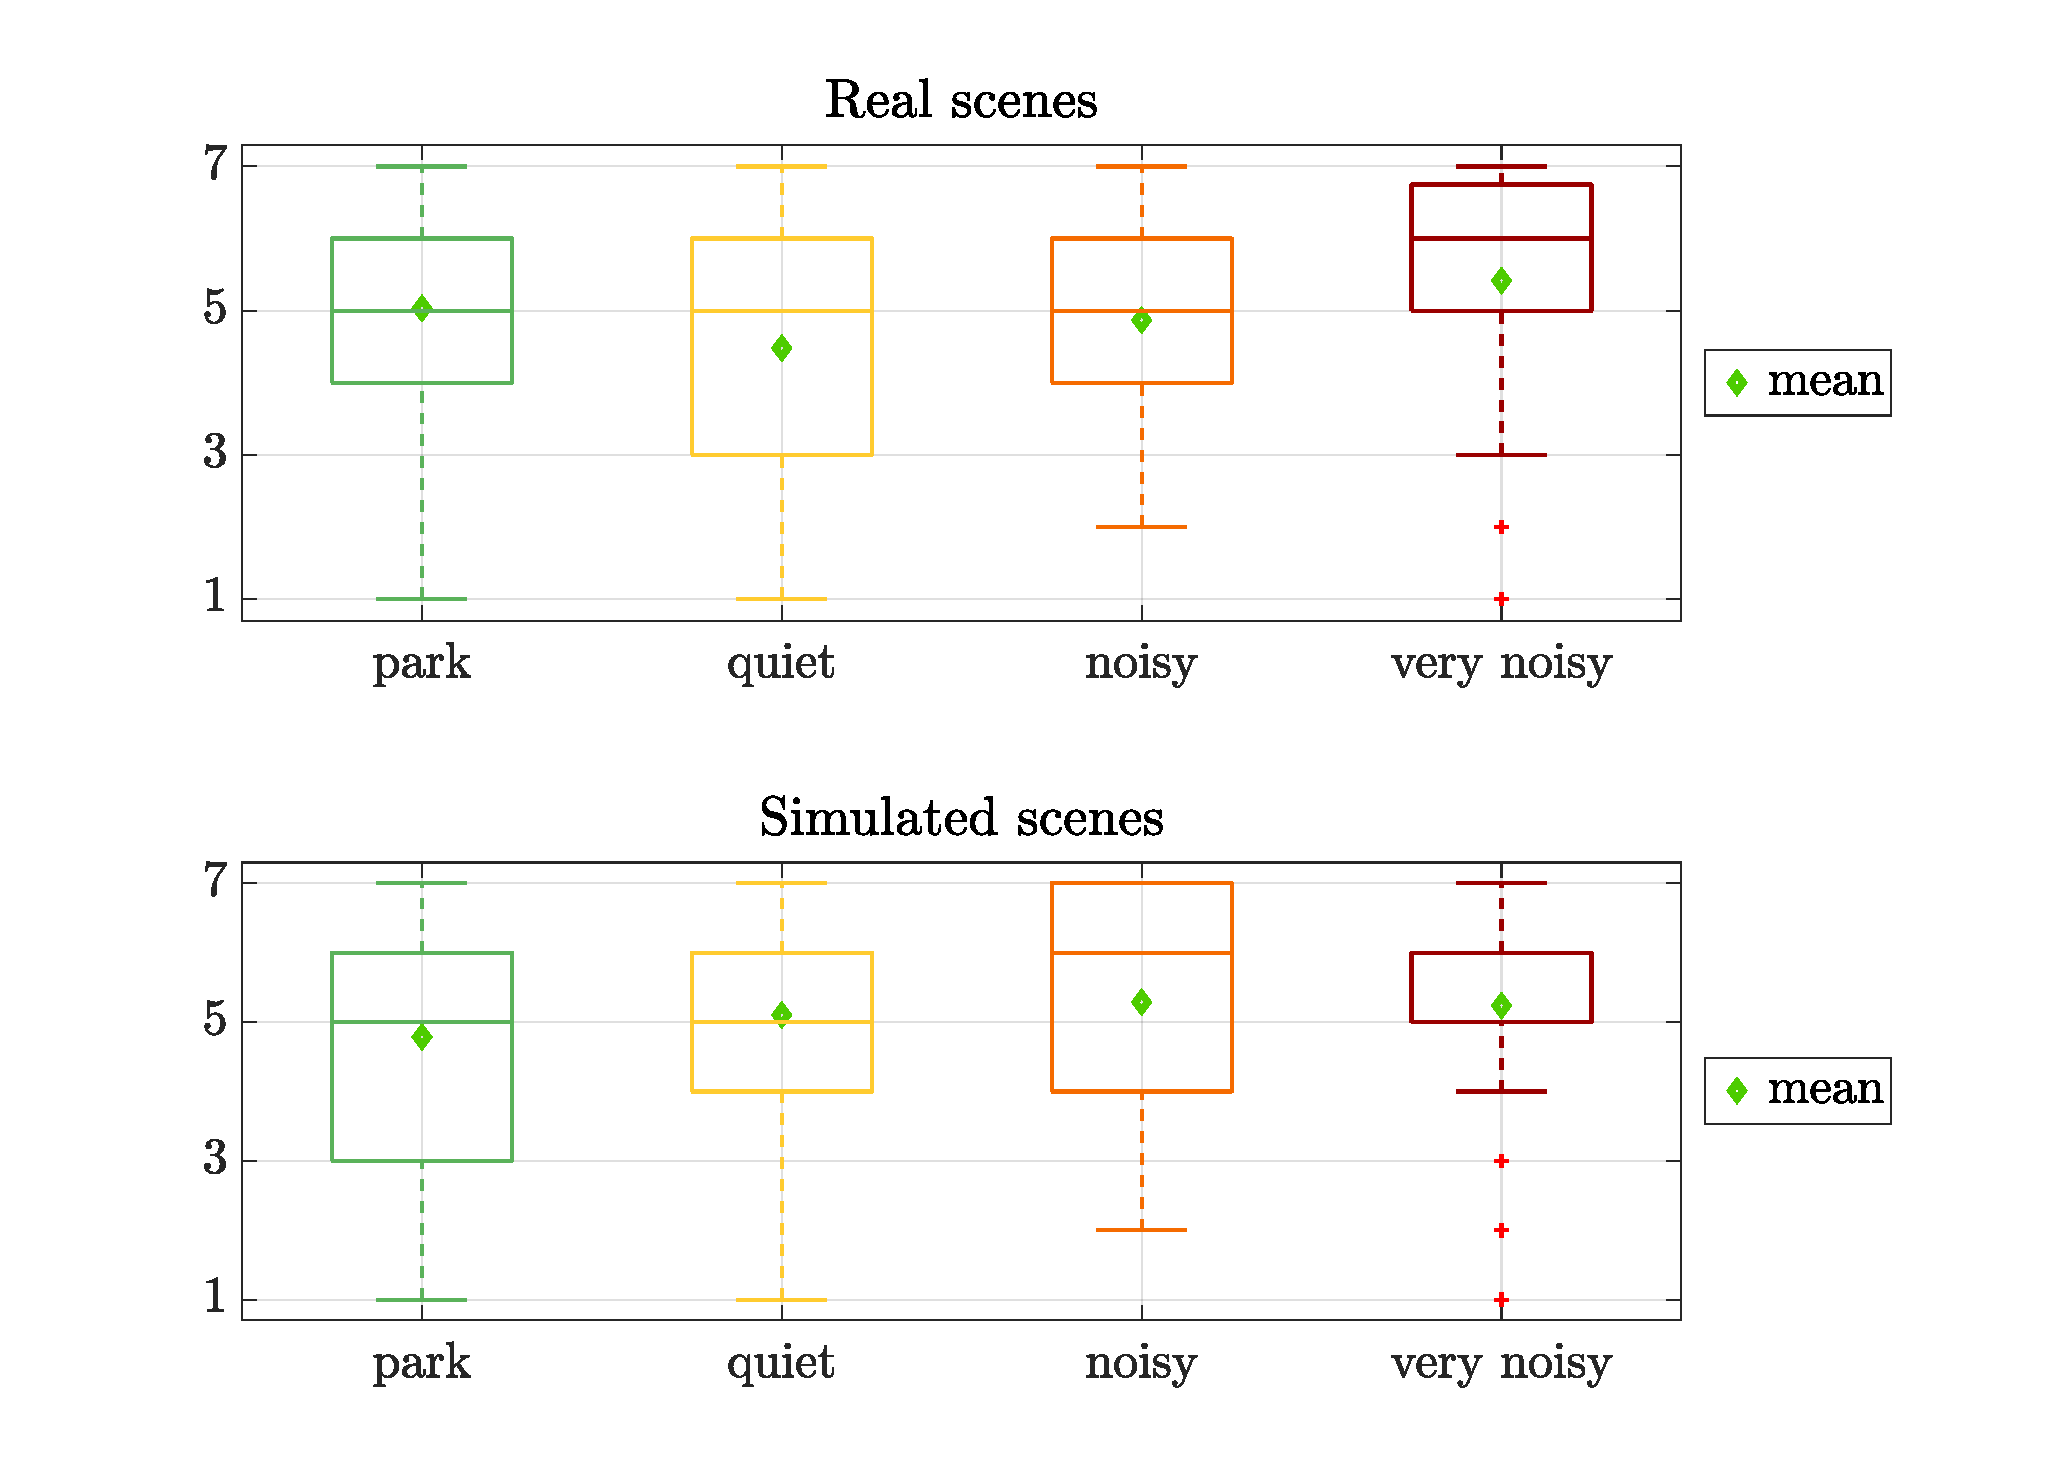
\includegraphics[width=.7\linewidth]{./pictures/testPerceptif_boxplotAmbianceCOLOR_EN.pdf}
\caption{Data distribution for the 'scene type' and 'sound environment' factors}
\label{fig:boxplot_type_ambience}
\end{figure}

\begin{table}[h]
\centering
\begin{tabular}{cccc}
        & DOF & \textit{F-statistic}    & \textit{p-value} \\ 
\hline
type & 1 & 1.38 & 0.24   \\
\hline
sound env.   & 3 & 4.69 & 3.60 $\times 10^{-3}$  \\ 
\hline
judge.   & 49 & 5 & 0.18 $\times 10^{-9}$  \\ 
\hline
type/sound env. & 3 & 6.80 & 0.20 $\times 10^{-3}$\\
\hline
type/judge & 49 & 1.07 & 0.35\\
\hline
sound env./judge & 147 & 1.43 & 1.60 $\times 10^{-3}$\\
\hline
\end{tabular}
\caption{Two-ways ANOVA for the 'type of sound' and 'sound environment' factors with the interaction effect}
\label{tab:p_value_type_ambience}
\end{table}


%Again, both the effects of each factors are not significant ($p-value > \alpha$) in contrast to its interaction ($p-value < \alpha$).  \\

Again, the 'type' factor is not influential in the distribution of the notes ($p-value > \alpha$) whereas the 'judge' and the 'sound environment' factors are. But most of all, interactions effects occur for the sound environment with respectively the 'type' factor and the 'judge' factors. The interaction effect can be easily illustrated for the case of the type and sound environment factors (figure \ref{fig:interaction}). It reveals that the perception of realism of the simulated and real scenes is not the same depending on the sound environment. 


\begin{figure}[hbtp]
\centering
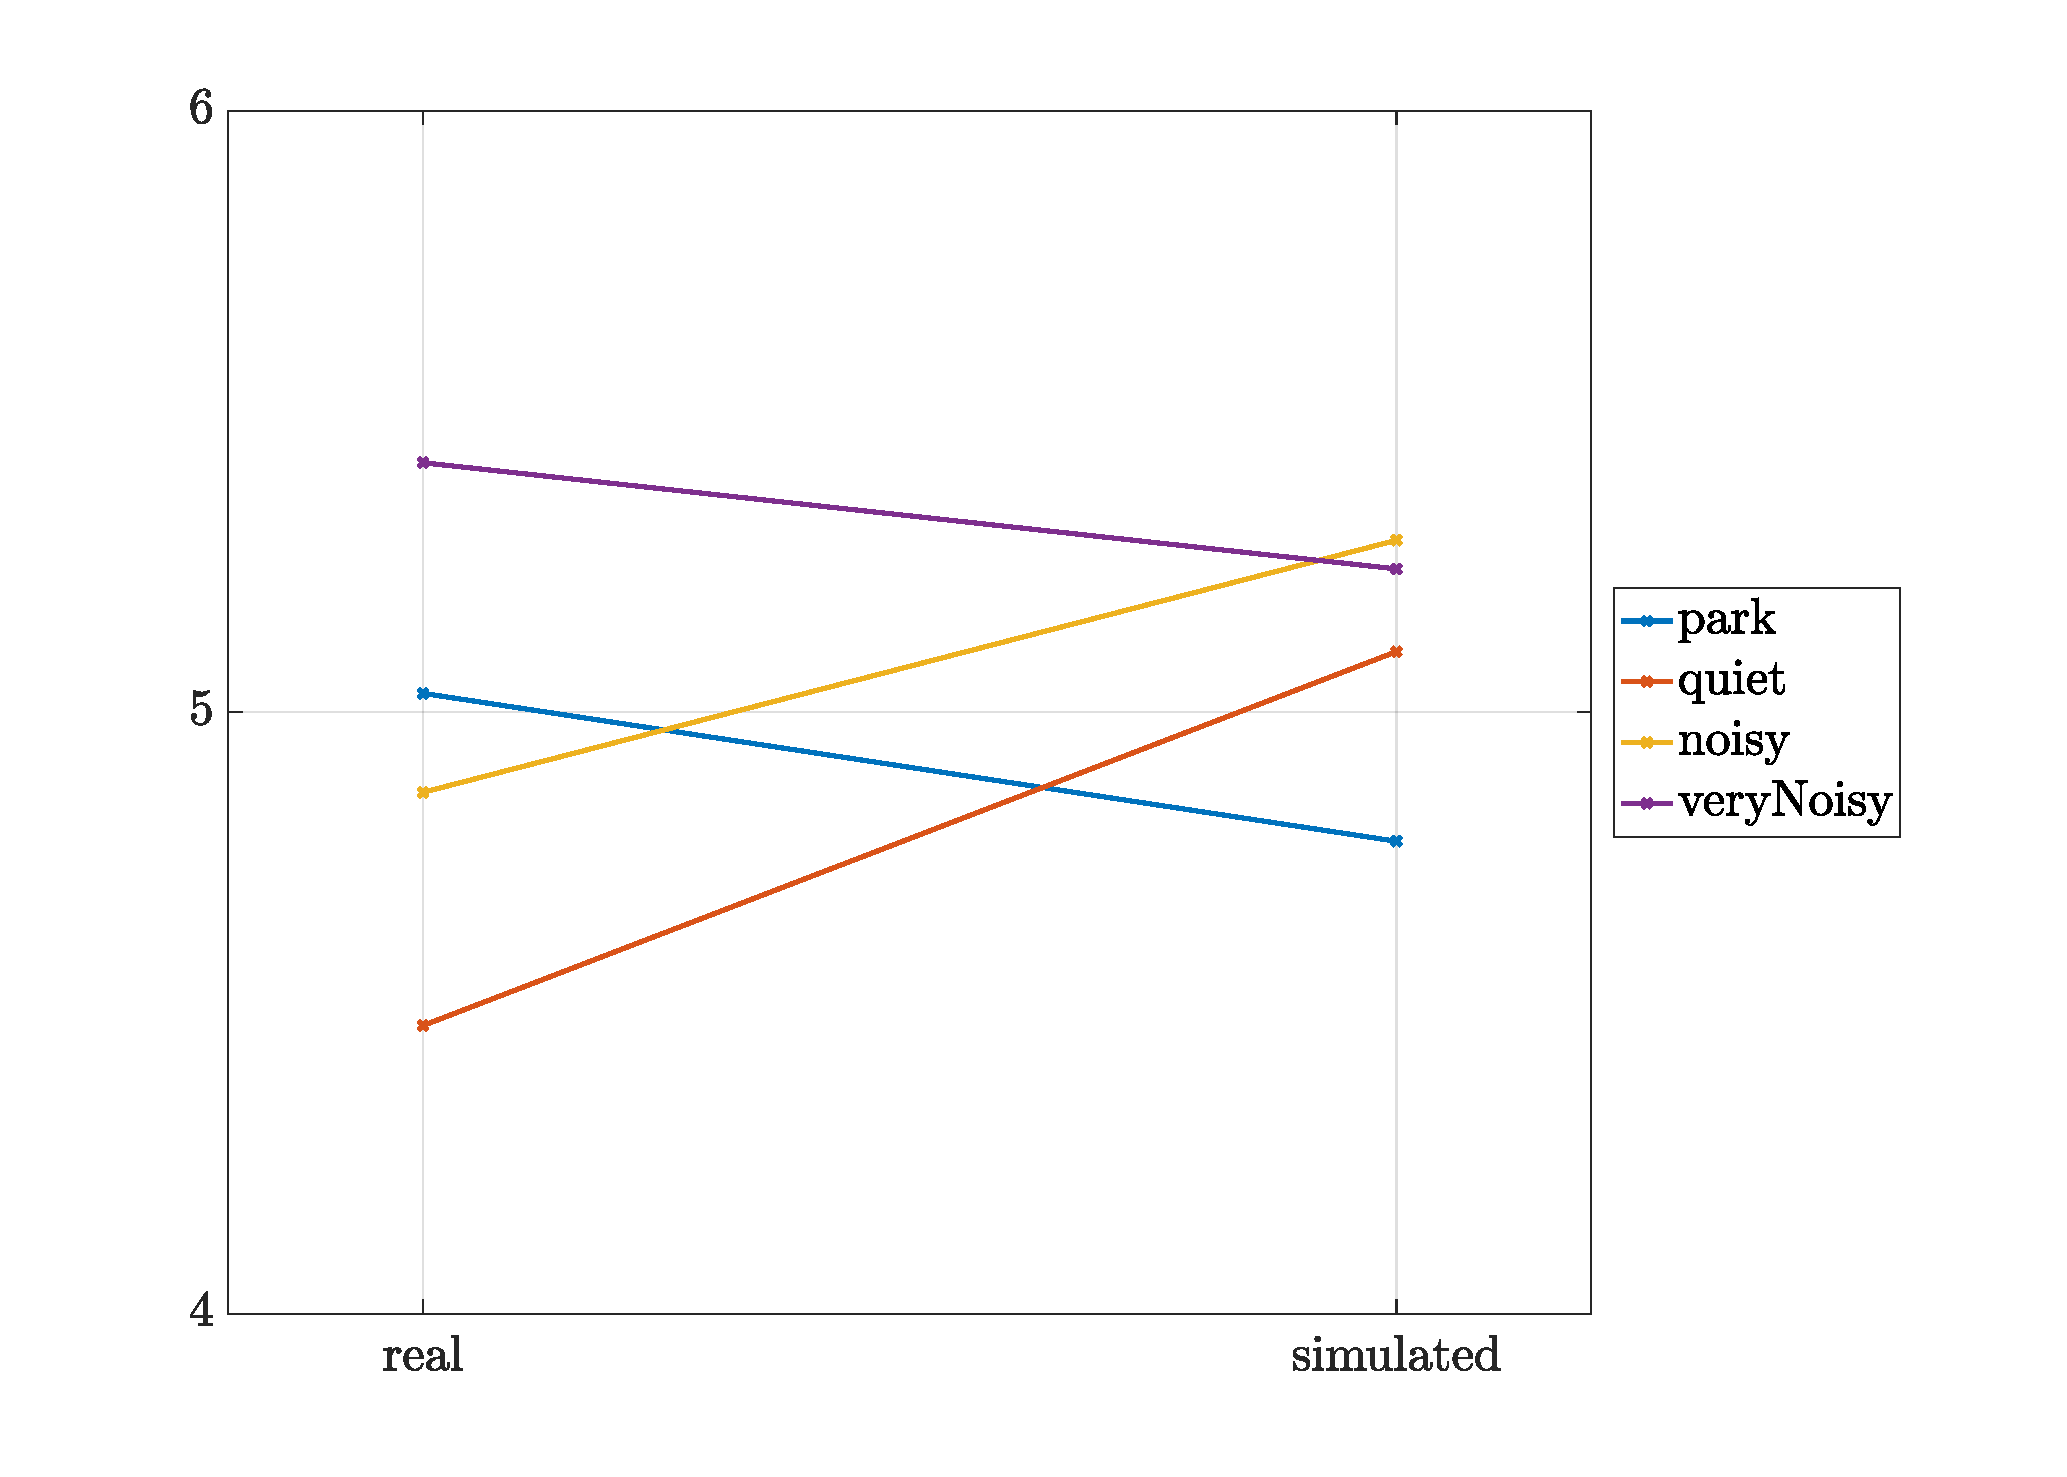
\includegraphics[width=.5\linewidth]{pictures/testPerceptif_interactionAmbianceCOLOR_EN.pdf}
\caption{Interaction of the two factors 'type of sound' and 'sound environment'}
\label{fig:interaction}
\end{figure}

For the \textit{quiet} and \textit{noisy} sound environments, the mean scores increase when the scenes are simulated whereas for the \textit{park} and \textit{very noisy} sound environment it decreases. As the effect of the \textit{type} factor is not the same according to the \textit{sound environment} levels, there is therefore an interaction effect. One notices that, on the simulated scenes, as the average scores of the \textit{noisy} and \textit{very noisy} atmospheres are higher for both, it seems that the presence of cars has been a preponderant element to increase the perceived realism of an audio mixture. On the contrary, for the \textit{quiet} and \textit{park} atmospheres, the evaluation is more complex. From the comments given by the subjects, it is mainly the sound class \textit{foot step} and a sound background composed of birds that have decreased the scene scores. In a similar way, in the real scenes, it is the presence of too loud birds and some street noises with unknown origins that have been remarked by the panelist and have degraded the evaluation.\\

\section{Conclusion}

In order to study the acoustic properties of the urban environment, the research community designs tools that have to be evaluated to demonstrate their merit. The availability of simulated scenes realistic enough with precise annotation in terms of content and level will foster research in this direction.

To do so, realistic urban sound mixtures have been composed from the analysis of urban recordings. A work of annotation has allowed to extract, for different acoustic atmospheres, some useful information as the sound classes presence, the traffic flow rates, the sound level. From these observations, a urban sound database has been created including multiple sound classes both for the sound events and backgrounds. As the road traffic is one of the most noise source, to have a full control on this, multiple car passages recordings have been made on a runway. A perceptual test has been set up to quantify the level of realism of the simulated scenes and has demonstrated that they are comparable to the recorded scenes. Then, the different ANOVA performed have demonstrated that, according to the judge and, most of all, to the sound environment factors, they may still be significant differences in the distribution of notes. In the \textit{park} and \textit{quiet street} environment, for the simulated scenes, the evaluations are more spread and the mean notes lower than the \textit{noisy} and \textit{very noisy} atmospheres. Theses differences come mainly from the sound level of some events which are found to be too loud to be realistic enough.

This problem solved, databases of sound sources and urban scenes can be shared with communities interested in methods of recognizing or detecting sound sources in order to help them to develop methods based on urban sound environments.

\section{Acknowledgements}
We would like to thank Pierre Aumond and Catherine Lavandier from the University of Cergy-Pontoise for transmitting us the data of the \textit{Grafic} project.

\bibliographystyle{unsrt}
\bibliography{bibliography}


\end{document}